\section{Introductory topics: particles and plasma in the Universe}\label{Introduction}
%{Introduction to cosmology and overview}
In this chapter, we will introduce the fundamental concepts in cosmology for us to explore the properties of the Universe during the `first hour'. I will first present the standard cosmological Friedmann-Lemaitre-Robertson-Walker (FLRW) model, then introduce the general Fermi/Bose distribution with and its application in the early Universe. Finally I present an overview of Universe evolution from $300\,\mathrm{MeV}>T>0.02\,\mathrm{MeV}$.
The Natural unit $c=\hbar=k_{B}=1$ is used throughout the thesis for discussion.
%{Introduction\daggerfootnote{This chapter has been published previously as \citet{Gottbrath1999}.}}

%~~~~~~~~~~~~~~~~~~~~~~~~~~~~~~~~~~~~~~~~~~~~~~~~~
%The modern observation in cosmology has demonstrated that the observed universe is highly symmetric in its large-scale structure and 

\subsection{Textbook review: the standard FLRW-Universe model}
%In this section we will focus on the following:
%\begin{itemize}
%    \item The Robertson –Walker Universe
%    \item The Friedmann equation (Hubble %    \item The composition of the universe
%\end{itemize}
The Friedmann-Lemaitre-Robertson-Walker (FLRW) Universe is a theoretical model used widely to describe the cosmological evolution of the Universe. It is based on the cosmological principles which assumes homogeneity and isotropy of the Universe on large scales. In general, the FLRW metric can be written as
\begin{align}\label{metric}
ds^2=c^2dt^2-a^2(t)\left[ \frac{dr^2}{1-kr^2}+r^2(d\theta^2+\sin^2\theta\,d\phi^2)\right].
\end{align}
The metric is characterized by the scale factor $a(t)$ which measures the size of the Universe as a function of time $t$. The geometric parameter $k$ identifies the Gaussian geometry of the spatial hyper-surfaces defined by co-moving observers. The metrics are qualitatively different depending on the value of $k$. We have $k=1$ which correspond to the closed Universe,  $k=0$ correspond to flat Universe, and $k=-1$ for open geometries of the Universe. Current observation of cosmic microwave background (CMB) anisotropy preferred value $k=0$~[\cite{Planck:2013pxb,Planck:2015fie,Planck:2018vyg}].


The cosmological equations that describe the evolution of the Universe are derived from the Einstein equations. In general, the Einstein equation with cosmological constant $\Lambda$ can be written as:
\begin{equation}\label{Einstein}
  G^{\mu\nu}=R^{\mu\nu}-\left(\frac R 2 +\Lambda\right) g^{\mu\nu}=8\pi G_N T^{\mu\nu}, 
\quad R= g_{\mu\nu}R^{\mu\nu}.  
\end{equation}
where $G_{N}$ is the Newtonian gravitational constant, and $T^{\mu\nu}$ is the stress-energy tensor. Given the homogeneous and isotropic symmetry conditions imply that the matter context of the Universe can be expressed as a perfect fluid. The stress-energy tensor $T^\mu_\nu$ of perfect fluid can be written as
\begin{align}
 T^\mu_\nu =\mathrm{diag}(\rho, -P, -P, -P).
\end{align}
where $\rho$ is energy density and an $P$ is the isotropic pressure.

Substituting the perfect fluid form of the stress-energy tensor into the Einstein equations, one can derive the cosmological equations that describe the evolution of the Universe. We then obtain Friedmann equations as follows:
\begin{align}
\label{Hubble} 
&H^{2}\equiv\left(\frac{\dot a}{a}\right)^2=\frac{8\pi G_{N}}{3}\rho-\frac{k}{a^2}+\frac{\Lambda}{3},\\
\label{q_value}
&qH^2=\frac{4\pi G_{N}}{3}\left(\rho+3P\right)-\frac{\Lambda}{3},\qquad q\equiv -\frac{a\ddot a}{\dot a^2},
\end{align}
where $H$ is the Hubble parameter,  $q$ is the deceleration parameter. These equations relate the dynamics of the scale factor $a(t)$ to the energy density and pressure of the cosmic plasma. On the other hand, considering the divergence freedom of the total stress-energy tensor $\nabla_\nu T^{\mu\nu}=0$. For $\mu=0$ component, we have
\begin{align}\label{energy_eq}
\nabla_\nu T^{0\nu}=\frac{d\rho}{dt}+3H(\rho+P)=0
\end{align}
which provides dynamical evolution equation for $\rho(t)$ and $P(t)$. Solutions of Eq.~(\ref{energy_eq}) describes the time evolution of  energy density and pressures in the Universe. Given the energy density and pressure as a function of time, we can illustrates how the Universe evolves according to the Friedmann equations Eq.~(\ref{Hubble}) and Eq.~(\ref{q_value}). Solving these equations allows us to understand the dynamics and evolution of the Universe such as the Hubble expansion and the behavior of matter and energy over cosmic time.





%~~~~~~~~~~~~~~~~~~~~~~~~~~~~~~~~~~~~~~~~~~~~~~~~~

\subsection{Approaching abundance equilibrium: Fermi/Bose distribution}

In the early Universe, the reaction rates of particles in the cosmic plasma were much greater than the Universe expansion rate $H$. Therefore, the local thermal equilibrium has been maintained. Assuming the particles are in thermal equilibrium, the dynamical information can be obtained from the single-particle distribution function. The general relativistic covariant Fermi/Bose momentum distribution can be written as
\begin{align}
f_{F/B}(\Upsilon_i,p_i)=\frac{1}{\Upsilon^{-1}_i\exp{\left[(u\cdot p_i-\mu_i)/T\right]}\pm1}
\end{align}
where the plus sign applies for fermions, and the minus sign for bosons. The Lorentz scalar $(u_i\cdot p_i)$ is a scalar product of the particle four momentum $p^\mu_i$ with the local four vector of velocity $u^\mu$. In the absence of local matter flow, the local rest frame is the laboratory frame 
\begin{align}
u^\mu=\left(1,\vec{0}\right),\,\,\,\,\,\,\,\,\, p^\mu_i=\left(E_i,\vec{p}_i\right).
\end{align}  
The parameter $\Upsilon_i$ is the fugacity of a given particle which describes the pair density and it is the same for both particles and antiparticles. For $\Upsilon_i=1$ the distribution maximizes the entropy content at a fixed particle energy. The parameter $\mu_i$ is the chemical potential for a given particle which is associated to the density difference between particles and antiparticles. 

In general there are two types of chemical equilibriums associated with the chemical parameters $\Upsilon$ and $\mu$. We have:
\begin{itemize}
\item Absolute chemical equilibrium:\\
The absolute chemical equilibrium is the level to which energy is shared into accessible degrees of freedom, e.g. the particles can be made as energy is converted into matter.
The absolute equilibrium is reached when the phase space occupancy approaches unity $\Upsilon\to1$. 
 \item Relative chemical equilibrium:\\
 The relative chemical equilibrium is associated with the chemical potential $\mu$ which involves reactions that distribute a certain already existent element/property among different accessible compounds. 
 \end{itemize}
The dynamics of absolute chemical equilibrium, in which energy can be converted to and from particles and antiparticles, is especially important. The consequences for the energy conversion to from particles/antiparticle can be seen in the first law of thermodynamics by introducing the general chemical potential $\mu_N$ for particle and $\mu_{\bar{N}}$ for antiparticle as follows:
\begin{align}
\mu_N\equiv\mu+T\ln\Upsilon,\qquad{\mu_{\bar{N}}}\equiv{-\mu}+T\ln\Upsilon.
\end{align}
Then the first law of thermodynamics can be written as
\begin{align}
dE&=-PdV+TdS+{\mu_N}dN+{\mu_{\bar{N}}}d{\bar{N}}
\\&=-PdV+TdS+{\mu}(dN-d{\bar{N}})+T\ln{\Upsilon}(dN+d{\bar{N}}).
\end{align}
It shows that the chemical potential $\mu$ is the energy required to change the difference between particles and antiparticles, and the $T\ln\Upsilon$ is the energy required to change the total number of particle and antiparticle, and the fugacity $\Upsilon$ is the parameter to adjust the energy.

\subsubsection{Boltzmann equation and particle freeze-out}
The Boltzmann equation describes the evolution of distribution function f in phase space. The Boltzmann equation in the FLRW universe can be written as
\begin{align}
\frac{\partial f}{\partial t}-\frac{\left(E^2-m^2\right)}{E}H\frac{\partial f}{\partial E}=\frac{1}{E}\sum_{q}\mathcal{C}_q[f],
\end{align}
where $H=\dot{a}/a$ is the Hubble parameter. Due to homogeneity and isotropy of the Universe, the distribution function depends on time $t$ and energy $E=\sqrt{p^2+m^2}$ only. The collision term $\sum_qC_q$ represents all elastic and inelastic interactions and $q$ labels the corresponding physical process. In general, the collision term is proportional to the relaxation time for given collision as follows [\cite{ANDERSON1974466}]
\begin{align}
\frac{1}{E}\mathcal{C}_q[f]\propto\frac{1}{\tau_{rel}}
\end{align}
where $\tau_{rel}$ is the relaxation time for the reaction, which is on the order of magnitude of time for the reaction to reach chemical equilibrium. 


As the Universe expands, the collision term in the Boltzmann equation competes with the Hubble term. In general, a given particle freeze-out from the cosmic plasma when its interaction rate $\tau_{rel}^{-1}$ becomes smaller than the Hubble expansion rate
\begin{align}
H\geqslant\tau_{rel}^{-1}.
\end{align}
When this happens, the particle's interactions are not rapid enough to maintain thermal distribution, either because the density of particles becomes so low that the chances of any two particles meeting each other becomes negligible, or because the particle energy becomes too low to interact. The freeze-out process can be categorized into three distinct stages based on the type of freeze-out interactions, we have~[\cite{Birrell:2012gg,Rafelski:2023emw}]:

\begin{itemize}
\item Chemical freeze-out :\\
As the Universe expands and the temperature drops, the rate of the inelastic scattering (e.g. production and annihilation reaction) that maintain the equilibrium density becomes smaller than the expansion rate. At this point, the inelastic scattering ceases, and a relic population of particles remain. Prior to the chemical freeze-out temperature, number changing processes are significant and keep the particle in thermal equilibrium, implying that the distribution function has the usual Fermi-Dirac form 
\begin{equation}\label{equilibrium}
f_{th}(t,E)=\frac{1}{\exp[(E-\mu)/T]+1},\qquad \text{ for } T(t)> T_{ch}.
\end{equation}
where $T_{ch}$ represents the chemical freeze-out temperature.


\item Kinetic freeze-out:\\
After chemical freeze-out, particles  still scatter elastically from other particles and keep thermal equilibrium in the primordial plasma. As the temperature drops, the rate of elastic scattering reaction that maintain the thermal equilibrium become smaller than the expansion rate. At that time, elastic scattering processes cease, and the relic particles do not interact with other particles in the primordial plasma anymore. Before the kinetic freeze-out, the distribution function has the form
\begin{equation}\label{kinetic_equilib}
f_k(t,E)=\frac{1}{\Upsilon^{-1}\exp[(E-\mu)/T]+1},\qquad \text{ for }T_f< T(t)< T_{ch},
\end{equation}
where $T_f$ represents the kinetic freeze-out temperature. The generalized fugacity $\Upsilon(t)$ controls the occupancy of phase space and is necessary once $T(t)<T_{ch}$ in order to conserve particle number.


\item{Free streaming:}\\
After kinetic freeze-out, the particles have fully decoupled from the primordial plasma, and thereby ceased influencing the dynamics of the Universe and become free-streaming. The Einstein-Vlasov equation can be solved [\cite{choquet2008general}] and the free-streaming momentum distribution can be written as [\cite{Birrell:2012gg}]
\begin{equation}\label{free_stream_dist}
f_{fs}(t,E)=\frac{1}{\Upsilon^{-1}\exp{\left[\sqrt{\frac{E^2-m^2}{T_{fs}^2}+\frac{m^2}{T^2_f}}-\frac{\mu}{T_f}\right]+1}},\quad T_{fs}(t)=\frac{T_fa(t_k)}{a(t)},
\end{equation}
where the free-streaming effective temperature $T_{fs}$ is obtained by redshifting the temperature at kinetic freeze-out. If a massive particle (e.g. dark matter) freeze-out from cosmic plasma in the nonrelativistic regime, $m\gg T_f$. We can use the
Boltzmann approximation, and the free-streaming distribution for nonrelativistic particle becomes
\begin{align}
&f^B_{fs}(t,p)=\Upsilon\,e^{-(m+\mu)/T_f}\exp\left[-\frac{1}{ T_{eff}}\frac{p^2}{2m}\right],\quad T_{eff}=\left(\frac{a(t_f)}{a(t)}\right)^2T_f,
\end{align}
where we define the effective temperature $T_{eff}$ for massive free-streaming particle. In this scenario, the effective temperature for massive particles decreases faster than the Universe temperature cools. It's worth emphasizing the different temperatures between cold free-streaming particles and hot cosmic plasma would affect the evolution of the early Universe and require more detailed study. 
\end{itemize}

The division of the freeze-out process into these three regimes is a simplification. However, it is a very useful approximation in the study of cosmology~[\cite{Mangano:2005cc,Birrell:2014gea}] . For detailed discussion, see [\cite{Birrell:2012gg,Rafelski:2023emw}].




\subsection{Thermodynamics of the Early Universe}
In the case of local thermal equilibrium, the laws of thermodynamics can provide a framework for understanding the behavior of particle's energy density, pressure, number density and entropy in the early Universe.

Using the relativistic covariant Fermi/Bose momentum distribution, the corresponding energy density, pressure, and number densities for particle species $i$ are given by
\begin{align}
\rho_i&=g_i\int\!\!\frac{d^3p}{(2\pi)^3}Ef_{F/B}=\frac{g_i}{2\pi^2}\!\int_{m_i}^\infty\!\!\!dE\,\frac{E^2\left(E^2-m_i^2\right)^{1/2}}{\Upsilon_i^{-1}e^{(E-\mu_i)/T}\pm 1},\label{energy_density}\\[0.2cm]
P_i&=g_i\int\!\!\frac{d^3p}{(2\pi)^3}\frac{p^2}{3E}f_{F/B}=\frac{g_i}{6\pi^2}\!\int_{m_i}^\infty\!\!\!dE\,\frac{\left(E^2-m_i^2\right)^{3/2}}{\Upsilon_i^{-1} e^{(E-\mu_i)/T}\pm 1},\label{Pressure_density}\\[0.2cm]
n_i&=g_i\int\!\!\frac{d^3p}{(2\pi)^3}f_{F/B}=\frac{g_i}{2\pi^2}\!\int_{m_i}^\infty\!\!\!dE\,\frac{E(E^2-m_i^2)^{1/2} }{\Upsilon_i^{-1}e^{(E-\mu_i)/T}\pm 1}
\label{number_density}
\end{align}
where $g_i$ is the degeneracy of the particle species. By including the fugacity parameter $\Upsilon_i$ allows us to characterize particle properties in nonchemical equilibrium situations.
On the other hand, the corresponding free-streaming energy density, pressure, and number densities can be written as
\begin{align}
\rho_i&=g_i\int\!\!\frac{d^3p}{(2\pi)^3}Ef_{fs}=\frac{g_i}{2\pi^2}\!\int_{m_i}^\infty\!\!\!dE\,\frac{E^2\left(E^2-m_i^2\right)^{1/2}}{\Upsilon_i^{-1}e^{\sqrt{p^2/T_{fs}^2+m_i^2 /T_f^2}-\mu_i/T_f}\pm 1},\label{free_energy_density}\\[0.2cm]
P_i&=g_i\int\!\!\frac{d^3p}{(2\pi)^3}\frac{p^2}{3E}f_{fs}=\frac{g_i}{6\pi^2}\!\int_{m_i}^\infty\!\!\!dE\,\frac{\left(E^2-m_i^2\right)^{3/2}}{\Upsilon_i^{-1}e^{\sqrt{p^2/T_{fs}^2+m_i^2 /T_f^2}-\mu_i/T_f}\pm1},\label{free_Pressure_density}\\[0.2cm]
n_i&=g_i\int\!\!\frac{d^3p}{(2\pi)^3}f_{fs}=\frac{g_i}{2\pi^2}\!\int_{m_i}^\infty\!\!\!dE\,\frac{E(E^2-m_i^2)^{1/2} }{\Upsilon_i^{-1}e^{\sqrt{p^2/T_{fs}^2+m_i^2 /T_f^2}-\mu_i/T_f}\pm1},
\label{free_number_density}
\end{align} 
which are different from the thermal equilibrium Eq.~(\ref{energy_density}), Eq.~(\ref{Pressure_density}), and Eq.~(\ref{number_density}), by replacing the mass by a time dependant effective mass $m\,T_{fs}(t)/T_f$ in the exponential.





Given the energy density, pressure, and number densities, the entropy density for particle species $i$ can be written as
\begin{align}\label{entropy}
\sigma_i=\frac{S_i}{V}=\left(\frac{\rho_i+P_i}{T}-\frac{\mu_i}{T}\,n_i\right).
\end{align}
In general the chemical potential is associated with the baryon number. Since the net baryon number density relative to the photon number density is of order $10^{-9}$. In this case, we can neglect the small chemical potential when calculating the total entropy density in the Universe. The total entropy density in the early Universe can be written as
\begin{align}
&\sigma=\sum_i\,\sigma_i=\frac{2\pi^2}{45}g^s_\ast\,T^3,\\
&g^s_\ast=\sum_{i=\mathrm{bosons}}g_i\left({\frac{T_i}{T_\gamma}}\right)^3B\left(\frac{m_i}{T_i}\right)+\frac{7}{8}\sum_{i=\mathrm{fermions}}g_i\left({\frac{T_i}{T_\gamma}}\right)^3F\left(\frac{m_i}{T_i}\right),
\end{align}
where $g^s_\ast$ counts the effective number of `entropy' degrees of freedom. The functions $B(m_i/T)$ and $F(m_i/T)$ are defined as
\begin{align}
&B\left(\frac{m_i}{T}\right)=\frac{45}{12\pi^4}\int^\infty_{m_i/T}\,dx\sqrt{x^2-\left(\frac{m_i}{T}\right)^2}\left[4x^2-\left(\frac{m_i}{T}\right)^2\right]\frac{1}{\Upsilon^{-1}_ie^x-1},\\
&F\left(\frac{m_i}{T}\right)=\frac{45}{12\pi^4}\frac{8}{7}\int^\infty_{m_i/T}\,dx\sqrt{x^2-\left(\frac{m_i}{T}\right)^2}\left[4x^2-\left(\frac{m_i}{T}\right)^2\right]\frac{1}{\Upsilon^{-1}_ie^x+1}.
\end{align}
In Fig.\,\ref{EntropyDOF_Fig} we plot the $g^s_\ast$ as a function of temperature, the effect of particle mass threshold~[\cite{Coc:2006rt}] is considered in the calculation for all involved particles. When $T$ decreases below the mass of particle $T\ll m_i$, this particle species becomes nonrelativistic and the contribution to $g^s_\ast$ becomes negligible, creating the dependence on $T$ seen in Fig.\,\ref{EntropyDOF_Fig}.
%~~~~~~~~~~~~~~~~~~~~~~~~~~~~~~~~~~~~~~~~~~~~~~~~~~~~~~~~~~~~~~~~~~~~~~~~~~~~~~~~
\begin{figure}[t]
%\begin{center}
\centering
\includegraphics[width=\linewidth]
%{./plots/DOF_entropy.jpg}
{./plots/g_entropy.jpg}
\caption{The entropy degrees of freedom as a function of $T$ in the early Universe epoch after hadronization $10^{-2}\,\mathrm{MeV} \leqslant  T \leqslant 150 $\,MeV. When particle species becomes nonrelativistic $T\ll m_i$, the contribution to $g^s_\ast$ becomes negligible, as a result creating the dependence $g^s_\ast(T)$.The vertical lines represents the mass of particles: $m_e=0.511$ MeV, $m_\mu=105.6$ MeV, and pion average mass $m_\pi\approx138$ MeV.}
\label{EntropyDOF_Fig}  
\end{figure}
%~~~~~~~~~~~~~~~~~~~~~~~~~~~~~~~~~~~~~~~~~~~~~~~~~~~~~~~~~~~~~~~~~~~~~~~~~~~~~~~~


\subsubsection{Relation between time and temperature}
Considering the comoving entropy conservation, we have
\begin{align}
S=\sigma V\propto g^s_\ast T^3a^3=\mathrm{constant},
\end{align}
where $g^s_\ast$ is the entropy degree of freedom and $a$ is the scale factor. Differentiating the entropy with respect to time $t$ we obtain
\begin{align}
\left[\frac{\dot{T}}{g^s_\ast}\frac{dg^s_\ast}{dT}+3\frac{\dot{T}}{T}+3\frac{\dot{a}}{a}\right]g^s_\ast T^3a^3=0,\qquad \dot{T}=\frac{dT}{dt}.
\end{align}
Solving $dT/dt$ and taking the integral, the relation between time and temperature in early universe can be written as
\begin{align}\label{time}
t(T)=t_0-\int^T_{T_0}dT\frac{1}{HT}\left[1+\frac{T}{3g^s_\ast}\frac{dg^s_\ast}{dT}\right],\qquad H^2=\frac{8\pi G_N}{3}\rho_{tot}
\end{align}
where $T_0$ and $t_0$ represent the initial temperature and time respectively, $H$ is the Hubble parameter and $\rho_{tot}$ is the total energy density in early Universe. From Eq. (\ref{time}) we see that the cosmic time depends on the entropy degrees of freedom $g^\ast_s$, which are characterized by the relativistic components in the early Universe. In the temperature range we consider $300\,\mathrm{MeV}>T>0.02\,\mathrm{MeV}$ the Universe is radiation-dominated and $\Lambda$CDM model is not used in this epoch.

%~~~~~~~~~~~~~~~~~~~~~~~~~~~~~~~~~~~~~~~~~~~~~~~~~~~~~~~~~~~~~~~$

\subsubsection{The baryon-per-entropy density ratio}
An important assumption allowing us to explore the early Universe evolution is that following on the era of matter genesis both baryon and entropy content is conserved in the comoving volume. Both baryon and entropy density scale with the third power of the expansion parameter $a(t)$. Therefore the ratio of baryon number density to visible matter entropy density remains constant throughout the evolution of universe. We have
\begin{align}
\frac{n_B-n_{\overline{B}}}{\sigma}= \left.\frac{n_B-n_{\overline{B}}}{ \sigma}\right|_{t_0}=\mathrm{Const.}\;
\end{align}
The subscript $t_0$ denotes the present day condition, and $\sigma$ is the total entropy density.
The observation gives the present baryon-to-photon ratio ~[\cite{ParticleDataGroup:2022pth}] $5.8 \times 10^{-10} \leqslant(n_B-n_{\overline{B}})/n_\gamma\leqslant6.5\times10^{-10}$. This small value quantifies the matter-antimatter asymmetry in the present day Universe, and allows the determination of the present value of baryon per entropy ratio~[\cite{Rafelski:2019twp,Fromerth:2002wb,Fromerth:2012fe}]:
\begin{align}\label{BaryonEntropyRatio}
\left.\frac{n_B-n_{\overline{B}}}{ \sigma}\right|_{t_0}=\eta\left(\frac{n_\gamma}{\sigma_\gamma+\sigma_\nu}\right)_{\!t_0}\!\!\!\!=(8.69\pm0.05)\!\!\times\!\!10^{-11},\qquad \eta=\frac{(n_B-n_{\overline{B}})}{n_\gamma},
\end{align}
where the $\eta=(6.12\pm0.04)\times10^{-10}$~[\cite{ParticleDataGroup:2022pth}] is used in calculation. To obtain the ratio, we consider that the Universe today is dominated by photons and free-streaming massless neutrinos~[\cite{Birrell:2012gg}], and $\sigma_\gamma$ and $\sigma_\nu$ are the entropy densities for photon and neutrino respectively. We have
\begin{align}
    \frac{\sigma_\nu}{\sigma_\gamma}=\frac{7}{8}\,\frac{g_\nu}{g_\gamma}\left(\frac{T_\nu}{T_\gamma}\right)^3\,\qquad\frac{T_\nu}{T_\gamma}=\left(\frac{4}{11}\right)^{1/3}
\end{align}
and the entropy-per-particle for massless bosons and fermions are given by~[\cite{Fromerth:2012fe}]
\begin{align}
s/n|_\mathrm{boson}\approx 3.60\,,\qquad
s/n|_\mathrm{fermion}\approx 4.20\,.
\end{align}
However, from the neutrino oscillation experiment, we know that the the neutrinos are not massless particles. 
The mass differences between neutrino mass eigenstates are~[\cite{ParticleDataGroup:2022pth}]:
\begin{align}
&\Delta{m}_{21}^2=7.39^{+0.21}_{-0.20}\times10^{-5}\,\mathrm{eV}^2,\\
&\Delta{m}_{32}^2=2.45^{+0.03}_{-0.03}\times10^{-3}\,\mathrm{eV}^2.
\end{align}
Neutrino mass eigenvalues can be ordered in the normal mass hierarchy ($m_1\ll m_2<m_3$) or inverted mass hierarchy ($m_3\ll m_1<m_2$). All three mass states remained relativistic until the temperature dropped below their rest mass. These results allow for the possibility that one mass eigenstate or two mass eigenstates of neutrinos may become non-relativistic today, which can affect the baryon-per-entropy ratio.




%~~~~~~~~~~~~~~~~~~~~~~~~~~~~~~~~~~~~~~~~~~~~~~~~~~~



\subsubsection{Nonequilibrium: departure from detailed balance}
Thermal equilibrium implies both chemical equilibrium (particles abundances are balanced) and kinetic equilibrium (energy is evenly distributed). In chemical equilibrium, the rates of the forward and reverse reactions are equal, resulting in a balance between production and annihilation/decay rates, which is called detailed balance. The chemical non-equilibrium can be achieved by breaking this detailed balance and leading to change in particle abundance over time. On the other hand, kinetic equilibrium is usually established much quicker and has less impact on the actual particle abundances.
The chemical nonequilibrium condition is more important than the kinetic equilibrium because it relates to the arrow of time for the particle reactions. 

The chemical nonequilibrium conditions in the early Universe are of general interest: they are understood to be prerequisite for the arrow of time dependent processes to take hold in the Hubble expanding Universe. The arrow of time plays an important role in the evolution of the early Universe, for example:
 1.) The Big Bang Nucleosynthesis (BBN)~[\cite{Pitrou:2018cgg,Kolb:1990vq,Dodelson:2003ft,Mukhanov:2005sc}]  the synthesis of light elements of  e.g. D, $^3$He, $^4$He, and $^7$Li are produced at temperatures around $86\,\mathrm{keV}>T_{BBN}>50\,\mathrm{keV}$. 
 2.) Baryogenesis is believed to occur at or before the Universe underwent electroweak phase transition~[\cite{Kolb:1990vq}] at a temperature $T\simeq 130$\, GeV, which generates the excess of baryon number compared to anti-baryon number in order to create the observed baryon number today.

When Universe expands and temperature cools down, the chemical non-equilibrium can be achieved by breaking the detailed balance between particle production reaction and annihilation/decay as follows:

1.) The particle production rate becomes slower than the rate of Universe expansion and the production reaction freezeout. Once the production reactions freezeout from the cosmic plasma, the corresponding detailed balance is broken and particle abundance decrease via the decay/annihilation reactions.
 

2.) The non-equilibrium can also be achieved when the production reaction slows down and is not able to keep up with decay/annihilation reaction. In this case, the Hubble expansion rate is much longer than the decay and production rate and is not relevant to the nonequilibrium process. The key factor is competition between production and decay/annihilation  which can result in chemical nonequilibrium in the early Universe.

\noindent We will investigate the nonequilibrium situation for bottom quarks and strang quarks in early universe and their application in Chapter~\ref{Bottom} and Chapter~\ref{Strangeness}, respectively.  

%~~~~~~~~~~~~~~~~~~~~~~~~~~~~~~~~~~~~~~~~~~~~~~~~~~~~~~~~~~~~~~~~~~



%~~~~~~~~~~~~~~~~~~~~~~~~~~~~~~~~~~~~~~~~~~~~~~~~~

\subsection{Cosmic plasma in early Universe $300\,\mathrm{MeV}>T>0.02\,\mathrm{MeV}$}
%In this section we will focus on the following:
%\begin{itemize}
%    \item Five different plasma epoch from $0.3\mathrm{GeV}>T>20$keV
%\end{itemize}

The primordial hot Universe fireball underwent several practically adiabatic phase changes that dramatically evolved its bulk properties as it expanded and cooled~[\cite{Rafelski:2023emw}]. We present an overview of the Universe evolution as a function of temperature from $300\,\mathrm{MeV}>T>0.02\,\mathrm{MeV}$ and main events constituting the history of the early Universe in Fig.~\ref{Overview_fig}. After the electroweak symmetry breaking epoch and presumably inflation, the comic plasma in the early Universe evolves in the following sequence:

%%%%%%%%%%%%%%%%%%%%%%%%%%%%%%%%%%%%%%%
\begin{figure}[ht]
 \centerline{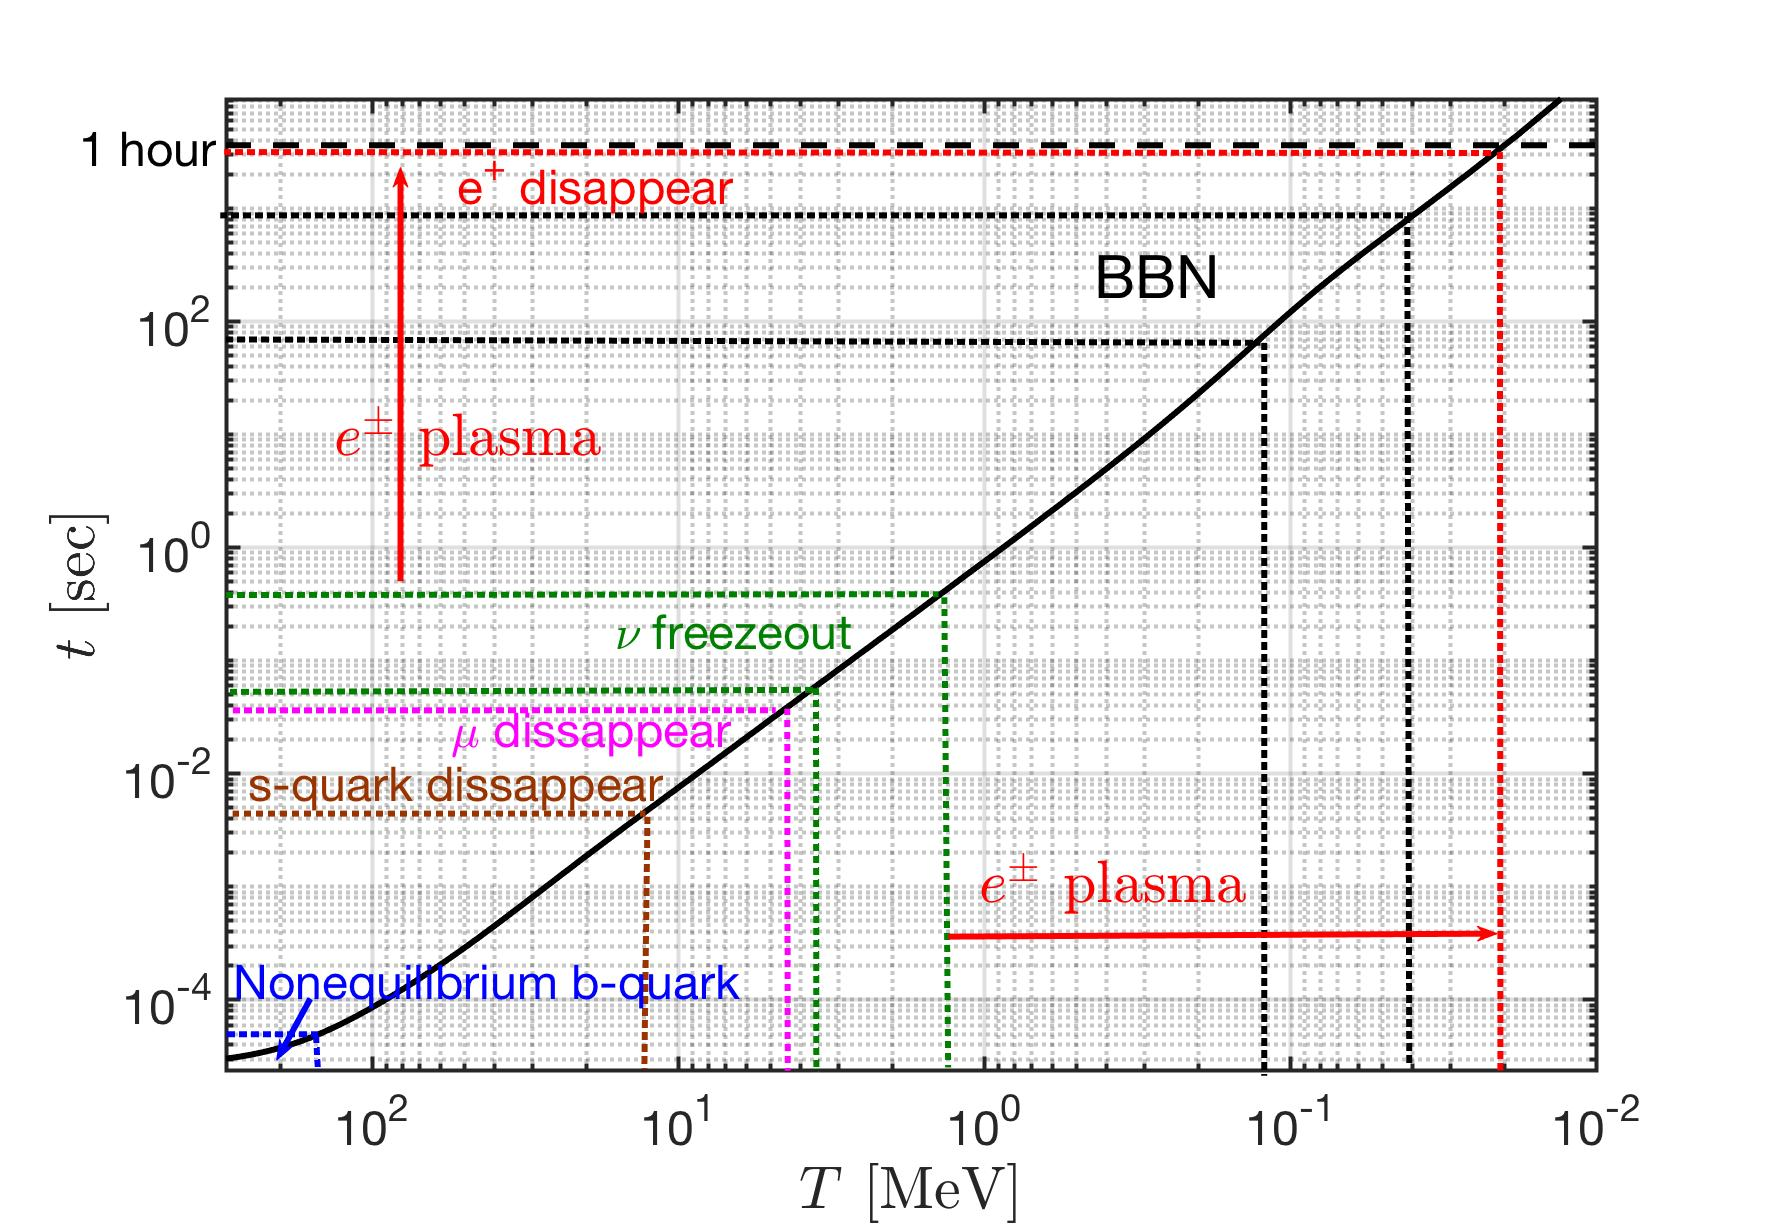
\includegraphics[width=\textwidth,width=\linewidth]{./plots/CosmicTimeTemperature_Project}}
 \caption{The time evolution of the early Universe as a function of temperature from $300\,\mathrm{MeV}>T>0.02\,\mathrm{MeV}$ and 
 different sequence of main events are shown with the temperature/time range in the evolution. }
 \label{Overview_fig}
\end{figure}
%%%%%%%%%%%%%%%%%%%%%%%%%%%%%%%%%%%%%%%

\begin{enumerate}
    \item \textbf{Primordial quark-gluon plasma}: 
    At early times when the temperature was between $130\,\mathrm{GeV}>T>0.15\,\mathrm{GeV}$ we have the building blocks of the Universe as we know them today, including the leptons, vector bosons, and all three families of deconfined quarks and gluons which propagated freely in plasma. As all hadrons are dissolved into their constituents during this time, strongly interacting particles $u,d,s,t,b,c,g$ controlled the fate of the Universe. When temperature is near to the QGP phase transition $300\, \mathrm{MeV}>T>150$ MeV, the bottom quark  breaks the detail balance and disappearance from particle inventory provides the arrow in time (see Chapter~\ref{Bottom} for detail).
    
    \item \textbf{Hadronic epoch}: Around the hadronization temperature $T_H\approx150\,\mathrm{MeV}$, a phase transformation occurred, forcing 
    the free quarks and gluons become confined within baryon and mesons [\cite{Letessier:2005qe}]. In the temperature range $ 150\,\mathrm{MeV}>T>20\,\mathrm{MeV}$, the Universe is rich in physics phenomena involving strange mesons and (anti)baryons including (anti)hyperon abundances~[\cite{Fromerth:2012fe,Yang:2021bko}]. The antibaryons disappear from the Universe at temperature $T=38.2$ MeV, and strangeness can be produced by the inverse decay reactions that are in equilibrium via weak, electromagnetic, and strong interactions in the early Universe until $T\approx13$ MeV (see Chapter~\ref{Strangeness} for detailed discussion).

    
    \item \textbf{Lepton-photon epoch}: For temperature $10\,\mathrm{MeV}>T>2\,\mathrm{MeV}$, the Universe contained relativistic electrons, positrons, photons, and three species of (anti)neutrinos. During this epoch massless leptons and photons controlled the fate of the Universe. Massive $\tau^\pm$ disappear from the plasma at high temperature via decay processes. However $\mu^\pm$ leptons can persist in the early Universe until temperature $T=4.2$ MeV, and positron $e^+$ can persist until the temperature $T=0.02$ MeV (See Chapter~\ref{Electron} for discussion).
    Neutrinos were still coupled to the charged leptons via the weak interaction~[\cite{Birrell:2012gg,Birrell:2014ona}] and freeze-out at temperature range $3\,\mathrm{MeV}>T>2\,\mathrm{MeV}$ which depends on the neutrino's flavors and the magnitude of the Standard Model parameters (See Chapter~\ref{Neutrino} for details). After neutrino freeze-out, they still play a important role in the Universe expansion via the effective number of neutrinos $N_{\nu}^{\mathrm{eff}}$ and affects the Hubble parameter significantly.  
    
    \item \textbf{Electron-positron epoch}: After neutrinos freeze-out at $T=3\sim2\,\mathrm{MeV}$ and become free-streaming in the early Universe, the cosmic plasma was dominated by electrons, positrons, and photons. The $e^\pm$ plasma existed until $T\approx0.02\,\mathrm{MeV}$ such that BBN occurred within a rich electron-positron plasma, and the dense number density of electron/positron also provide the opportunities to investigate magnetization process (See Chapter~\ref{Electron} for detailed discussion). This is the last time the Universe will contain a significant fraction of its content in antimatter.
\end{enumerate}
After $e^\pm$ annihilation, the Universe was still opaque to photons at this point and remained so until the recombination period at $T\approx0.25\,\mathrm{eV}$ starting the era of observational cosmology with the Cosmic Microwave Background. This period has been studied in detail before in~[\cite{Planck:2018vyg}]. Therefore, we focus on the temperature $300\,\mathrm{MeV}>T>0.02\,\mathrm{MeV}$ which corresponds to the first hour of the Universe evolution. We will address the cosmic plasma as follow: In Chapter~\ref{Bottom}, we discuss the heavy quarks (bottom/charm) abundance near to the QGP hadronization and show the nonequilibrium of bottom quark.  In Chapter~\ref{Strangeness} we study the strangeness abundance after hadronization and show the long lasting strangeness in the early Universe. In Chapter~\ref{Neutrino} we focus on the neutrino-matter interactions and the evolution of cosmic neutrino in early universe before/after freeze-out. In Chapter~\ref{Electron} we study the abundance of charged leptons $\mu^\pm$ and $e^\pm$ and show that the present of $e^\pm$ plasma plays an important role in early Universe. In Chapter~\ref{Outlook} we address the ongoing and prospective research projects for future publication.
Finally in Chapter~\ref{Summary} we summarize the important results of our study and conclusion.
%~~~~~~~~~~~~~~~~~~~~~~~~~~~~~~~~~~~~~~~~~~~~~~~~~



%\begin{figure}
%\centering
%\includegraphics[angle=0,width=\columnwidth]{fig1.pdf}
%\caption[]{}
%\label{fig1}
%\end{figure}